\documentclass[12pt]{exam}
\usepackage[utf8]{inputenc}

\usepackage{amsmath,amstext,amsthm,amssymb,amsxtra,cancel}
\usepackage[top=1.5in, bottom=1.5in, left=1.25in, right=1.25in]	{geometry}
%\usepackage[normalem]{ulem}
\usepackage{txfonts} % pxfonts txfonts 
\usepackage[T1]{fontenc}
\usepackage{lmodern}
\renewcommand*\familydefault{\sfdefault}
 \usepackage{euler}   % better than the option below
\usepackage{pdfsync}
\usepackage{multicol}
\newcommand{\ci}[1]{_{ {}_{\scriptstyle #1}}}
\usepackage{graphicx}
\graphicspath{ {images/} }


\newcommand{\norm}[1]{\ensuremath{\left\|#1\right\|}}
\newcommand{\abs}[1]{\ensuremath{\left\vert#1\right\vert}}
\newcommand{\ip}[2]{\ensuremath{\left\langle#1,#2\right\rangle}}
\newcommand{\p}{\ensuremath{\partial}}
\newcommand{\pr}{\mathcal{P}}

\newcommand{\pbar}{\ensuremath{\bar{\partial}}}
\newcommand{\db}{\overline\partial}
\newcommand{\D}{\mathbb{D}}
\newcommand{\B}{\mathbb{B}}
\newcommand{\Sp}{\mathbb{S}}
\newcommand{\T}{\mathbb{T}}
\newcommand{\R}{\mathbb{R}}
\newcommand{\Z}{\mathbb{Z}}
\newcommand{\C}{\mathbb{C}}
\newcommand{\N}{\mathbb{N}}
\newcommand{\Q}{\mathbb{Q}}
\newcommand{\mQ}{\mathcal{Q}}
\newcommand{\mS}{\mathcal{S}}
\newcommand{\scrH}{\mathcal{H}}
\newcommand{\scrL}{\mathcal{L}}
\newcommand{\td}{\widetilde\Delta}
\newcommand{\pw}{\text{PW}}
\newcommand{\esup}{\text{ess.sup}}
\newcommand{\Tn}{\mathcal{T}_n}
\newcommand{\Bn}{\mathbb{B}_n}
\newcommand{\rt}{\mathcal{O}}
\newcommand{\avg}[1]{\langle #1 \rangle}
\newcommand{\one}{\mathbbm{1}}
\newcommand{\eps}{\varepsilon}
\newcommand{\grad}{\nabla}

\newcommand{\La}{\langle }
\newcommand{\Ra}{\rangle }
\newcommand{\rk}{\operatorname{rk}}
\newcommand{\card}{\operatorname{card}}
\newcommand{\ran}{\operatorname{Ran}}
\newcommand{\osc}{\operatorname{OSC}}
\newcommand{\im}{\operatorname{Im}}
\newcommand{\re}{\operatorname{Re}}
\newcommand{\tr}{\operatorname{tr}}
\newcommand{\vf}{\varphi}
\newcommand{\f}[2]{\ensuremath{\frac{#1}{#2}}}

\newcommand{\kzp}{k_z^{(p,\alpha)}}
\newcommand{\klp}{k_{\lambda_i}^{(p,\alpha)}}
\newcommand{\TTp}{\mathcal{T}_p}
\newcommand{\m}[1]{\mathcal{#1}}
\newcommand{\md}{\mathcal{D}}
\newcommand{\qan}{\abs{Q}^{\alpha/n}}
\newcommand{\sbump}[2]{[[ #1,#2 ]]}
\newcommand{\mbump}[2]{\lceil #1,#2 \rceil}
\newcommand{\cbump}[2]{\lfloor #1,#2 \rfloor}

\newcommand{\hn}{{4 }}
\newcommand{\dd}{{June 21}}
\newcommand{\class}{Math 412 Summer 23}
\newcommand{\term}{Spring 2022}
\newcommand{\examnum}{Homework \hn: Due \dd}
\newcommand{\examdate}{}
\newcommand{\timelimit}{75 Minutes}
\newcommand{\vc}[3]{\langle #1,#2,#3\rangle}
\newcommand*{\vv}[1]{\vec{\mkern0mu#1}}
\newcommand{\bv}[1]{\boldsymbol{#1}}
\newcommand{\hide}[1]{}
\newcommand{\uvec}[1]{\boldsymbol{\hat{\textbf{#1}}}}
\newcommand{\vex}[1]{\boldsymbol{{\textbf{#1}}}}
\newcommand{\px}{\partial_x}
\newcommand{\py}{\partial_y}
\newcommand{\pt}{\partial_t}
\newcommand{\pxx}{\partial_{xx}}
\newcommand{\pyy}{\partial_{yy}}
\newcommand{\ptt}{\partial_{tt}}


\pagestyle{head}
\firstpageheader{}{}{}
\runningheader{\class}{ Page \thepage\ of \numpages}{\examnum}
\runningheadrule

\makeatletter
\renewcommand*\env@matrix[1][*\c@MaxMatrixCols c]{%
  \hskip -\arraycolsep
  \let\@ifnextchar\new@ifnextchar
  \array{#1}}
\makeatother

%\printanswers
\begin{document}

\noindent
\begin{tabular*}{\textwidth}{l @{\extracolsep{\fill}} r @{\extracolsep{6pt}} l}
\textbf{\class} & \textbf{Name:} & \textbf{Benjamin Tollison}\\
\end{tabular*}\\
\rule[2ex]{\textwidth}{2pt}
%

 

This is homework number \hn and it is \textbf{due on \dd}. You \textit{must} use this template for your
homework. You can either print it out and write on it and upload that, or you can use a tablet
if you have one. Alternatively, I am providing you with a link the the \LaTeX template. If you 
type your homework then (1) you'll become accustomed to using \LaTeX which is probably good 
and (2) you'll get a bonus of 2 points (each HW assignment is 10 points, so this means that
your maximum is 12 if you type). Whichever you choose, you will turn it in on Gradescope. 

Also, no matter which method you choose, your work must be neat, legible, and must flow clearly. This,
of course, includes the requirement that you show you work appropriately. 
See examples in class of what I am looking for. In particular, there should be nothing that is 
scratched out (either use Whiteout or something similar or just re-write the whole thing). The
work should more or less progress from left to right, top to bottom. In short, imagine that this
is a history class or something and you're turning in your \textit{final draft}. Part of what you 
are being graded on is your ability to communicate well which, at a minimum, means the reader can 
actually read what you have written.

Three of the problems will be graded
for accuracy, the others will be graded for ``completion''. Here, ``completion'' means: is it 
clear the student made an honest attempt at the problem and wrote the solution/attempt up in a
neat way?


\newpage 
\begin{questions}
\begin{question}
Solve $\pt u + u \px u = 0$ on $x\in (-\infty,\infty)$ and $t>0$ if 
$u(x,0) = \begin{cases}1, & 0<x<2\\ 0, & \textnormal{else}\end{cases}$.
\end{question}
\begin{solutionorbox}[\stretch{1}]
\end{solutionorbox}

\newpage 
\begin{question}
For a conservation equation $\pt u + \px f(u) = 0$, the solution is shown below for $t=0$ on the left and for 
a generic $0<t<t_1$ on the right: 

\begin{minipage}{.484\linewidth}
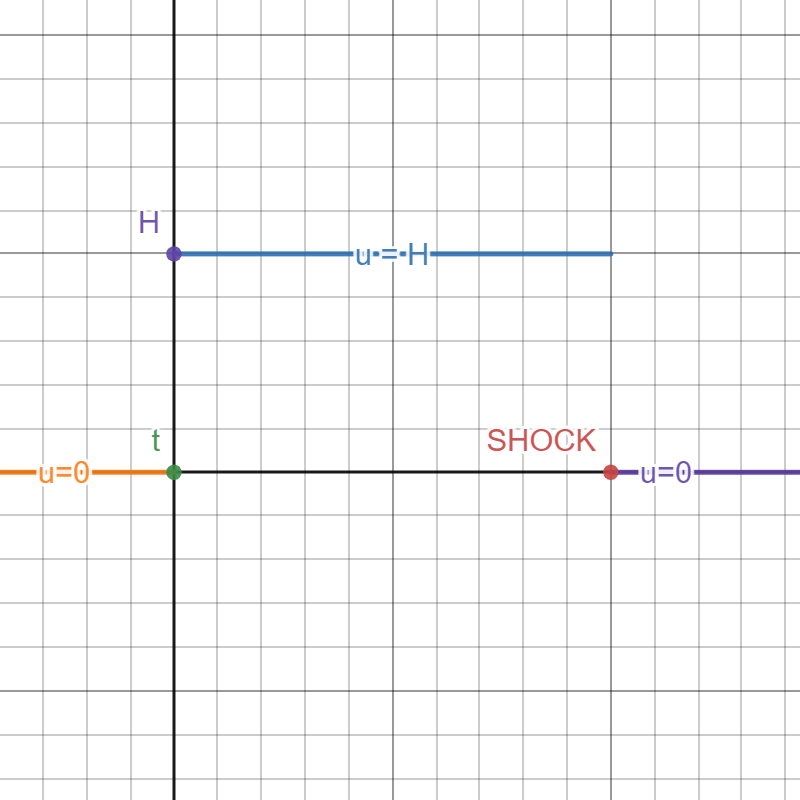
\includegraphics[width=.9\linewidth]{graph27.png}
\end{minipage}
\begin{minipage}{.484\linewidth}
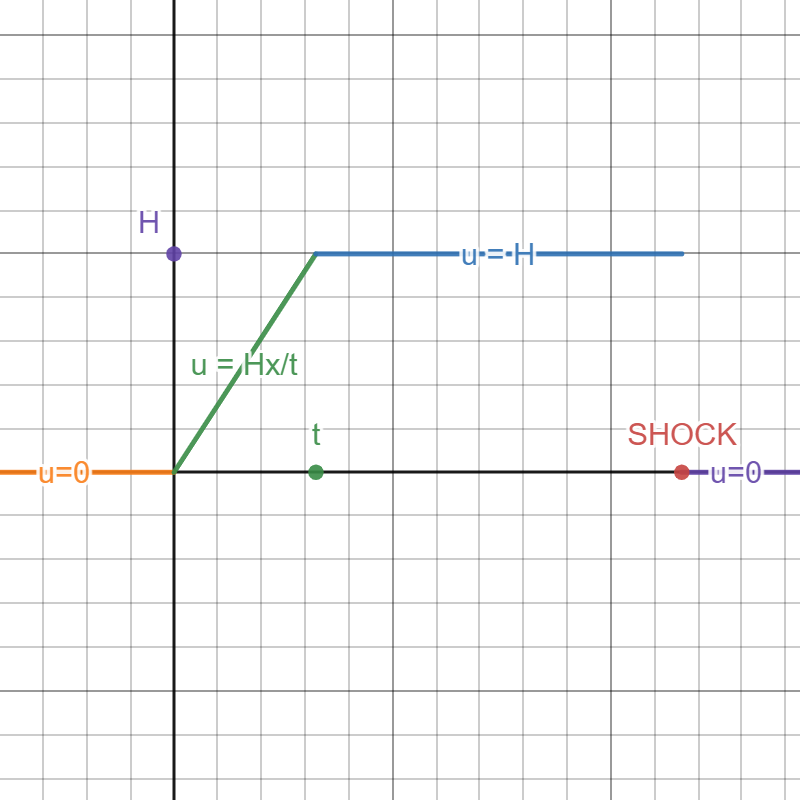
\includegraphics[width=.9\linewidth]{graph26.png}
\end{minipage}

Use this to answer the following questions: 
\begin{enumerate}
    \item Find a formula for $x_S(t)$ -- the shock location (this is the "SHOCK" label in the diagram). 
    \item At some value of $t$, this value for the shock will no longer be correct. What is that value?
    \item Compute $[q]$ -- the jump in $q$ across the shock. 
\end{enumerate}


\end{question}
\begin{solutionorbox}[\stretch{1}]
\end{solutionorbox}


\newpage 
\begin{question}
Show (by differentiating) that the Alembert Solution solves the wave equation. For ease of notation, take 
$c^2 = 1$. 
\end{question}
\begin{solutionorbox}[\stretch{1}]
\end{solutionorbox}


\newpage 
\begin{question}
Solve $\ptt u = \pxx u$ if $u(x,0) = \sin x$ and $\pt u(x,0) = x$.
\end{question}
\begin{solutionorbox}[\stretch{1}]
\end{solutionorbox}

\newpage 
\begin{question}
Solve $\pxx u - 3\px\pt u - 4\ptt u = 0$ if $u(x,0) = x^2$ and $\pt u(x,0)=e^x$.
\end{question}
\begin{solutionorbox}[\stretch{1}]
\end{solutionorbox}
\end{questions}
\end{document}
